\newpage
\section{The Process}
process: 流程
\subsection{A Generic Process Model}
\begin{figure}[!htb]
    \centering
    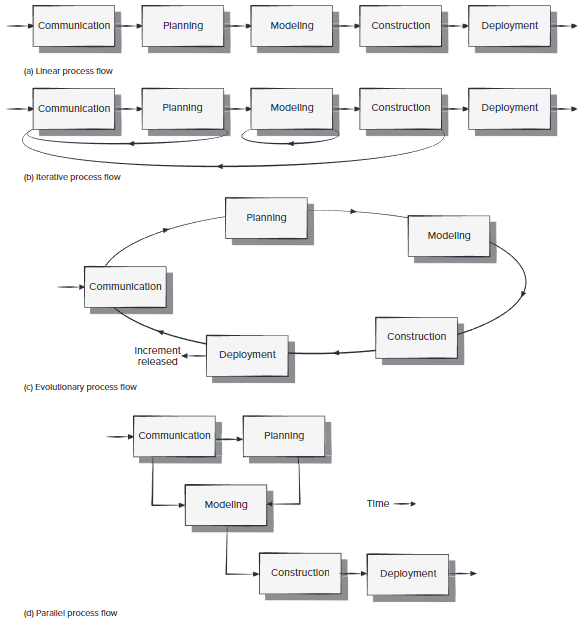
\includegraphics[width=0.42\textwidth]{pic/SE2/Process flow}
    \caption{Process flow}
\end{figure}

\subsection{Process Patterns}

\subsection{Process Assessment and Improvement}



\subsection[CMMI]{The Capability Maturity Model Integration}
\begin{itemize}
    \item Level 0: Incomplete
    \item Level 1: Performed(无序)
    \item Level 2: Managed(模板化, 组织化)
    \item Level 3: Defined(系统化)
    \item Level 4: Quantitatively managed(量化)
    \item Level 5: Optimized
\end{itemize}

\subsection{Prescriptive Process Models}

\begin{itemize}
    \item The Waterfall Model
    \begin{figure}[!htb]
        \centering
        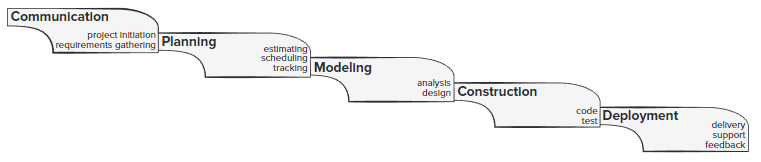
\includegraphics[width=0.42\textwidth]{pic/SE2/The Waterfall Model}
        \caption{The Waterfall Model}
    \end{figure}
    \item V-model
    \item The Incremental Model
    \item Prototyping Process Model
    \begin{figure}[!htb]
        \centering
        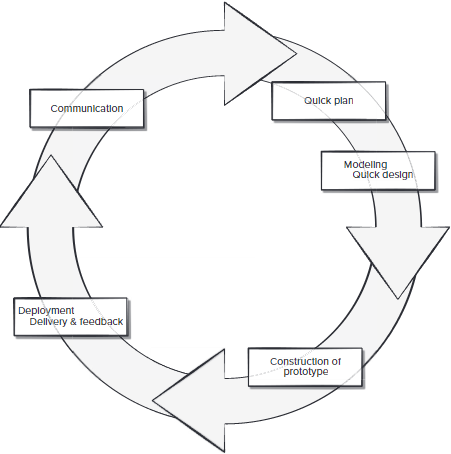
\includegraphics[width=0.309\textwidth]{pic/SE2/The prototyping paradigm}
        \caption{The prototyping paradigm}
    \end{figure}
    
    \item Evolutionary Process Model
    \begin{figure}[!htb]
        \centering
        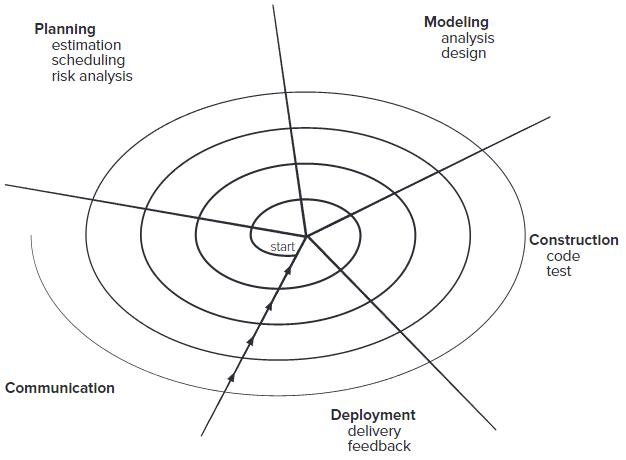
\includegraphics[width=0.309\textwidth]{pic/SE2/A typical spiral model}
        \caption{A typical spiral model}
    \end{figure}
    
    \item Unified Process Model(UML)
    \begin{figure}[!htb]
        \centering
        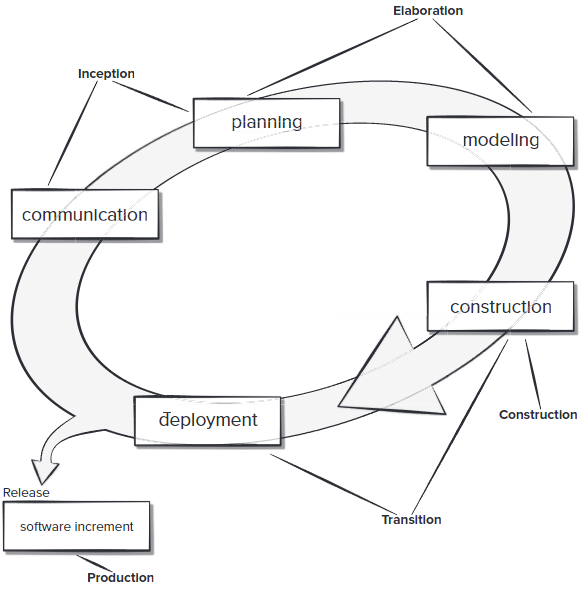
\includegraphics[width=0.309\textwidth]{pic/SE2/The Unified Process}
        \caption{The Unified Process}
    \end{figure}
    
\end{itemize}



